% !TEX encoding = UTF-8
% !TEX TS-program = pdflatex
% !TEX root = ../tesi.tex

%**************************************************************
\chapter{Analisi dei requisiti}
\label{cap:analisi-requisiti}

\section{Analisi del problema}
Per risolvere il problema descritto in nella descrizione del progetto\riferimento{sec:progetto}, ovvero l'automazione della configurazione del motore semantico di Engagent, ho scomposto tale problema nei seguenti \textit{macro-task}, quindi ho studiato come automatizzarli:
\begin{enumerate}
    \item \textbf{creazione delle \emph{regole}\glsfirstoccur};
    \item \textbf{creazione dei synset};
    \item \textbf{raffinamento dei risultati};
    \item \textbf{creazione del file di configurazione \emph{NLP} per il motore semantico};
\end{enumerate}

\subsection*{Creazione delle regole}\label{creazione_regole}
Questo task è il più difficile da automatizzare, perché richiede la definizione di \emph{match} contenenti categorie correlate tra loro. Inoltre, non esistono delle regole uguali per tutti, ma ogni settore ha regole diverse.\\
La soluzione è stata trovata nell'intelligenza artificiale, più in particolare nel clustering. Tramite l'analisi di \emph{chat} e \textit{FAQ}\glsfirstoccur{} archiviate, è possibile generare delle regole allo stato grezzo.\\
Rimane il problema della bassa affidabilità dei risultati. Possibili soluzioni:
\begin{itemize}
    \item \textbf{più dati in input:} non realizzabile nel breve periodo;
    \item \textbf{algoritmo più complesso:} task attribuito a ricercatori esterni all'azienda;
    \item \textbf{raffinamento manuale dei risultati:} richiede meno tempo rispetto alla creazione dell'NLP da zero. Questa soluzione è la più semplice nel breve periodo; 
    \item \textbf{raffinamento automatico dei risultati:} buon compromesso tra il raffinamento manuale e le altre due soluzioni.
\end{itemize}

\subsection*{Creazione dei synset}
La creazione dei \emph{synset} è automatizzabile trovando i sinonimi delle categorie che compongono le regole. Ho scomposto questo \textit{macro-task} nei seguenti \textit{task}:
\begin{itemize}
    \item estrazione delle parole che compongono le regole in una lista;
    \item portare la parola a una forma standard (attraverso TreeTagger);
    \item per ogni parola, trovare i suoi sinonimi (attraverso \textit{NLTK Wordnet}).
\end{itemize}

\subsection*{Raffinamento dei risultati}
I risultati dell'algoritmo di clustering devono essere ripuliti da \emph{stop words}\glsfirstoccur e regole prive di significato.
Le \textit{stop words} sono una lista di parole che non possono far parte del modello, definite da \company{}.
Una regola è significativa quando permette di individuare un gruppo di domande con lo stesso significato. 

\subsection*{creazione del modello NLP}
La creazione del modello per il motore semantico di Engagent richiede di aver creato delle regole e \emph{synset} corretti. Inoltre, per garantire flessibilità all'applicazione, è necessario permettere la manipolazione del modello attraverso l'aggiunta, la modifica e la rimozione di elementi in ogni momento.



%**************************************************************
\section{Casi d'uso}
Ho preceduto la progettazione dell'applicazione dalla stesura dei casi d'uso, supportati da diagrammi dei casi d'uso coerenti con lo standard UML.\\
I casi d'uso sono aumentati durante tutta la durata dello stage. Durante lo sviluppo, assieme al tutor, abbiamo individuato nuove funzionalità per raffinare i risultati e migliorare l'automazione di \app{}.

\begin{usecase}{0}{Scenario principale}
\usecaseactors{Utente}
\usecasepre{Il sistema è stato installato correttamente. L'utente ha aperto una \textit{shell} posizionata nella root dell'applicazione. (stato principale del sistema)}
\usecasedesc{Il sistema, tramite CLI (\textit{command line interface}), permette di:
    \begin{itemize}
        \item 1 inserire un file json;
        \item 2 inserire un file xlsx;
        \item 3 personalizzare i parametri in output;
        \item 4 attivare o disattivare le funzionalità del programma;
        \item 5 creare una configurazione per il motore semantico di Engagent;
        \item 6 caricare automaticamente l'output in Engagent; 
        \item 7 inserire in input una configurazione già esistente;
        \item 8 utilizzo dell'applicazione attraverso una \textit{REST API};
        \item 9 visualizzazione delle informazione di esecuzione del sistema (\textit{log}).
    \end{itemize}
}
\begin{figure}[H]
    \centering 
    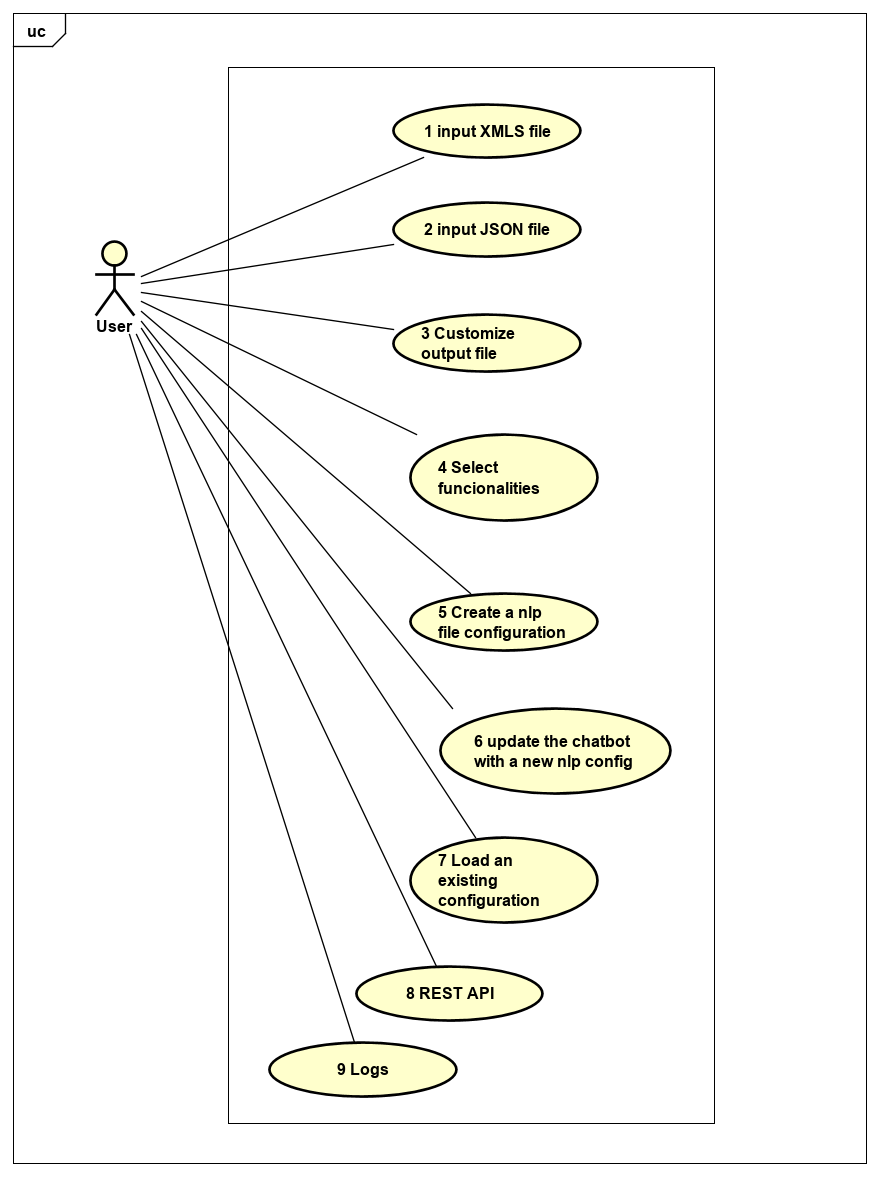
\includegraphics[width=0.9\columnwidth]{usecase/general_view.png} 
    \caption{Use Case - UC0: Scenario principale}
\end{figure}

\usecasepost{Il sistema è pronto per una nuova iterazione}
\label{uc:scenario-principale}
\end{usecase}

\begin{usecase}{1/2}{inserire un file json/xlsx}
    \usecaseactors{Utente}
    \usecasepre{Il sistema mette a disposizione un comando per l'input di un file json/xlsx}
    \usecasedesc{L'utente, tramite CLI, inserisce un file json/xlsx}
    \usecasepost{Il sistema permette di inserire un nuovo file in input}
    \label{uc:1/2}
\end{usecase}

\begin{usecase}{3}{Personalizzazione parametri in output}
    \usecaseactors{Utente}
    \usecasepre{Il sistema mette a disposizione dei comandi per la personalizzazione dell'output}
    \usecasedesc{L'utente, tramite CLI, personalizza i parametri di output:
    \begin{itemize}
        \item 3.1 modifica del dominio;
        \item 3.2 modifica della lingua;
        \item 3.3 modifica dei prefissi;
        \item 3.4 modifica della priorità delle regole.
    \end{itemize}
    }
    \usecasepost{Il sistema torna allo stato principale}
    \label{uc:3}
\end{usecase}

\begin{figure}[H]
    \centering 
    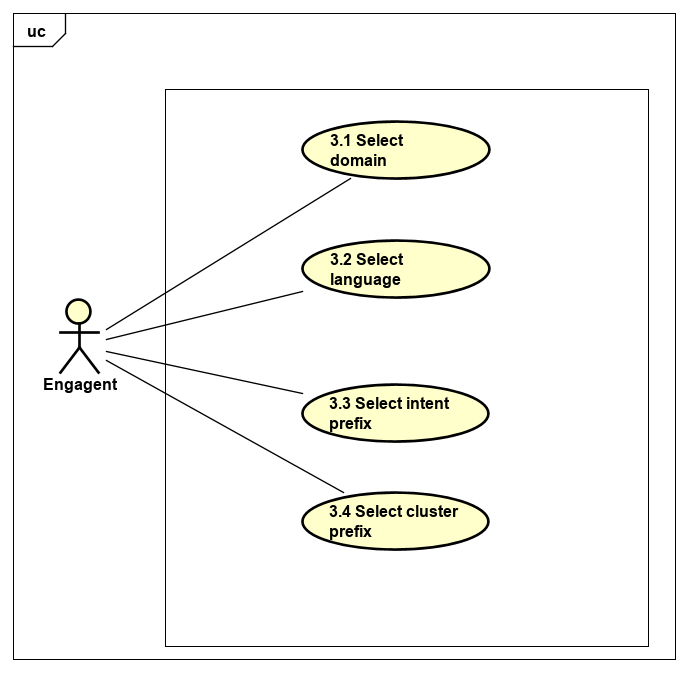
\includegraphics[width=0.7\columnwidth]{usecase/customize_output.png} 
    \caption{Use Case - UC3: Personalizzazione parametri in output}
\end{figure}

\begin{usecase}{3.1, 3.2, 3.3, 3.4}{Personalizzazione dominio/lingua/prefissi/priorità delle regole}
    \usecaseactors{Utente}
    \usecasepre{Il sistema mette a disposizione dei comandi per la personalizzazione dell'output}
    \usecasedesc{L'utente, tramite CLI, modifica il dominio/lingua/prefissi/priorità delle regole}
    \usecasepost{Il sistema permette di personalizzare nuovi parametri}
    \label{uc:3.1/3.2/3.3/3.4}
\end{usecase}

\begin{usecase}{4}{funzionalità del programma}
    \usecaseactors{Utente}
    \usecasepre{Il sistema mette a disposizione dei comandi per selezionare quali funzionalità del programma utilizzare}
    \usecasedesc{L'utente, tramite CLI, attiva o disattiva le seguenti funzionalità:
    \begin{itemize}
        \item 4.1 stemming sulle categorie;
        \item 4.2 validazione delle categorie attraverso le domande associate;
        \item 4.3 rimozione delle stop words\glsfirstoccur{};
        \item 4.4 creazione di \textit{cluster};
        \item 4.5 creazione di \textit{intent}.
    \end{itemize}
    }
    \usecasepost{Il sistema torna allo stato principale}
    \label{uc:4}
\end{usecase}

\begin{usecase}{4.1}{Stemming sulle categorie}
    \usecaseactors{Utente}
    \usecasepre{Il sistema mette a disposizione dei comandi per l'attivazione (o disattivazione) dello stemming. Lo stemming consiste nell'estrazione della radice da una parola.}
    \usecasedesc{L'utente, tramite CLI, attiva o disattiva lo stemming}
    \usecasepost{Il sistema permette all'utente di modificare altre funzionalità}
    \label{uc:4.1}
\end{usecase}

\begin{usecase}{4.2}{Validazione delle categorie attraverso le domande associate}
    \usecaseactors{Utente}
    \usecasepre{Il sistema mette a disposizione dei comandi per l'attivazione (o disattivazione) della validazione delle categorie. Questa funzione permette di filtrare le categorie, escludendo quelle assenti nelle domande associate, aumentando la precisione del risultato.}
    \usecasedesc{L'utente, tramite CLI, attiva o disattiva la validazione delle categorie}
    \usecasepost{Il sistema permette all'utente di modificare altre funzionalità}
    \label{uc:4.2}
\end{usecase}

\begin{usecase}{4.3}{rimozione delle \textit{stop words}}
    \usecaseactors{Utente}
    \usecasepre{Il sistema mette a disposizione dei comandi per l'attivazione (o disattivazione) del filtro delle \textit{stop words}. Le stop words sono delle parole che il sistema deve ignorare durante l'esecuzione del programma.}
    \usecasedesc{L'utente, tramite CLI, attiva o disattiva il filtro delle stop words}
    \usecasepost{Il sistema permette all'utente di modificare altre funzionalità}
    \label{uc:4.3}
\end{usecase}

\begin{usecase}{4.4}{Creazione dei cluster}
    \usecaseactors{Utente}
    \usecasepre{Il sistema mette a disposizione dei comandi per l'attivazione (o disattivazione) della creazione dei \textit{cluster}. I \textit{cluster} devono essere definiti nel file di input.}
    \usecasedesc{L'utente, tramite CLI, attiva o disattiva la creazione dei cluster}
    \usecasepost{Il sistema permette all'utente di modificare altre funzionalità}
    \label{uc:4.4}
\end{usecase}

\begin{usecase}{4.5}{Creazione degli intent}
    \usecaseactors{Utente}
    \usecasepre{Il sistema mette a disposizione dei comandi per l'attivazione (o disattivazione) della creazione degli \textit{intent}. Un intent è una regola composta da un singolo match.}
    \usecasedesc{L'utente, tramite CLI, attiva o disattiva la creazione degli intent}
    \usecasepost{Il sistema permette all'utente di modificare altre funzionalità}
    \label{uc:4.5}
\end{usecase}

\begin{usecase}{5}{Creare una configurazione compatibile con il motore semantico di Engagent}
    \usecaseactors{Utente}
    \usecasepre{Il sistema mette a disposizione un comando per la creazione della configurazione}
    \usecasedesc{L'utente, tramite CLI, crea una nuova configurazione}
    \usecasepost{\'E stato creato un nuovo file contenente la configurazione. Il sistema è tornato allo stato principale}
    \label{uc:5}
\end{usecase}
\begin{usecase}{6}{Caricare automaticamente la configurazione in Engagent}
    \usecaseactors{Utente}
    \usecasepre{Il sistema mette a disposizione un comando per caricare automaticamente il file contenente la configurare in Engagent}
    \usecasedesc{L'utente, tramite CLI, carica il file contenente la configurazione in Engagent}
    \usecasepost{Engagent contiene la nuova configurazione}
    \label{uc:6}
\end{usecase}
\begin{usecase}{7}{Inserire una configurazione già esistente}
    \usecaseactors{Utente}
    \usecasepre{Il sistema mette a disposizione un comando per l'input di una configurazione già esistente (vengono ereditate \textit{regole} e \textit{synset})}
    \usecasedesc{L'utente, tramite CLI, carica una configurazione esistente}
    \usecasepost{Il sistema contiene la configurazione di partenza}
    \label{uc:7}
\end{usecase}

\begin{usecase}{8}{Utilizzo dell'applicazione attraverso una \textit{REST API}}
    \usecaseactors{Utente}
    \usecasepre{L'applicazione espone dei comandi REST per l'esecuzione dell'applicazione in remoto}
    \usecasedesc{L'utente esegue dei comandi REST indirizzati a un server remoto}
    \usecasepost{Il sistema permette l'esecuzione di nuovi comandi REST}
    \label{uc:8}
\end{usecase}

\begin{usecase}{9}{visualizzazione delle log}
    \usecaseactors{Utente}
    \usecasepre{L'applicazione permette la generazione dei \textit{log} durante l'esecuzione}
    \usecasedesc{L'utente esegue l'applicazione}
    \usecasepost{Il sistema genera automaticamente i \textit{log} e li salva in un \textit{database}}
    \label{uc:9}
\end{usecase}

\section{Tracciamento dei requisiti}

Da un'attenta analisi dei requisiti e degli use case effettuata sul progetto è stata stilata la tabella che traccia i requisiti in rapporto agli use case.\\
Il codice dei requisiti è così strutturato R[O/D][F/V][Num. requisito] dove:
\begin{enumerate}
	\item[R =] requisito
    \item[O =] obbligatorio
    \item[D =] desiderabile
    \item[F =] Funzionale
    \item[V =] Vincolo 
\end{enumerate}

\label{tab:requisiti-funzionali}
\begin{table}[H]
\centering
\resizebox{\textwidth}{!}{
\begin{tabular}{|l l l|}
\hline
\textbf{Requisito} & \textbf{Descrizione} & \textbf{Fonte} \\
\hline
ROF-1     & L'utente può inserire un file Excel & UC1 \\
ROF-2     & L'utente può inserire un file Json & UC2 \\
ROF-3     & L'utente può personalizzare la configurazione & UC3 \\
ROF-3.1   & L'utente può modificare il dominio della configurazione & UC3.1 \\
ROF-3.2   & L'utente può modificare la lingua della configurazione & UC3.2 \\
ROF-3.3   & L'utente può modificare i prefissi delle regole nella configurazione & UC 3.3\\
ROF-3.4   & L'utente può modificare le priorità dei match nella configurazione & UC3.4 \\
ROF-4     & L'utente può attivare o disattivare le funzionalità del programma & UC4 \\
ROF-4.1   & L'utente eseguire lo stemming\glsfirstoccur{} sulle categorie & UC4.1 \\
ROF-4.2   & Validazione delle categorie, attraverso le frasi associate & UC4.2 \\
ROF-4.3   & L'utente filtrare le \textit{stop words} & UC4.3 \\
ROF-4.4   & L'utente può creare i \textit{cluster} & UC4.4 \\
ROF-4.5   & L'utente creare gli \textit{intent} & UC4.5 \\
ROF-5     & L'utente può creare un file contenente la configurazione & UC5\\
RDF-1     & creazione di una configurazione estendendone una già esistente & UC7 \\
RDF-2     & caricare automaticamente una configurazione in \textit{Engagent} & UC6 \\
RDF-3     & L'applicazione deve esporre un servizio REST API & UC8 \\
RDF-4     & L'applicazione genera i \textit{log}& UC9 \\
\hline
\end{tabular}
}
\caption{Tracciamento dei requisiti funzionali}
\end{table}\label{tab:requisiti-funzionali-fine} 

\label{tab:requisiti-vincolo}
\begin{table}[H]
\resizebox{\textwidth}{!}{
\begin{tabular}{|l l l|}
\hline
\textbf{Requisito} & \textbf{Descrizione} & \textbf{Fonte} \\
\hline
ROV-1     & le funzioni più importanti devono essere riutilizzabili & Tutor aziendale\\
ROV-2     & L'applicazione deve essere sviluppata in Python 3.7 & Tutor aziendale \\
ROV-3     & esecuzione in tempo lineare rispetto alla grandezza del file & Tutor aziendale \\
ROV-4     & Il codice deve essere coperto da almeno 80\% di test di unità & Tutor aziendale \\
ROV-5     & Il codice deve rispettare lo stile pep8 & Obiettivo personale \\
\hline
\end{tabular}
}
\caption{Tracciamento dei requisiti di vincolo}
\end{table}